We present two different case studies that illustrate the results of the refinement algorithm. 

\subsection{Belief liveness + task specification}
Figure \ref{fig:case1} shows a gridworld divided into 'rooms'. The agent needs to patrol the green cell . Additionally, the agent has to 'see' the target or constrain its belief of the target to 1 cell infinitely often i.e, the surveillance specification is $\square \lozenge p_1 \wedge \square \lozenge goal$ where the goal is the green cell. 

\begin{figure}
\centering
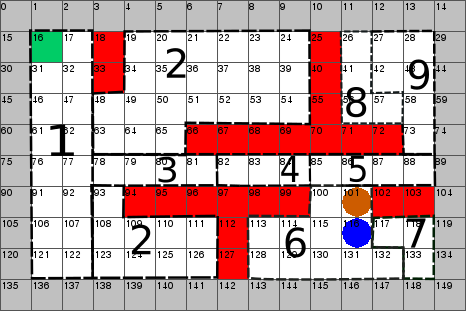
\includegraphics[scale=0.4]{text970.png}\caption{Gridworld with refined 9 abstract states after 5 iterations of refinement.}\label{fig:case1}
\vspace{-.5cm}
\end{figure}

\begin{table}[h!]
\begin{tabular}{c|c|c|c}
& Not refined & Partially refined & Fully refined \\ \hline \hline
Number of states & 104 & 616 & $2\times10^{31}$
\end{tabular}
\end{table}
The refinement algorithm terminates after 5 iterations to produce the abstract partition $\mathcal{Q} = \{Q_1,...,Q_9 \}$ corresponding to the numbered sets in figure \ref{fig:case1}. There are 9 belief states which results in an additional $2^9 = 512$ states to the full observation game which is far lower than the full reduction which will be a power set of all 104 states.

 A video simulation can be found at \textbf{LINK}. Note the behaviour of the agent going to the target and then searching for the target. This will contrast with the behaviour under belief safety specifications which are be looked at next. 

\subsection{Belief safety + task specification}
\begin{figure}
\centering
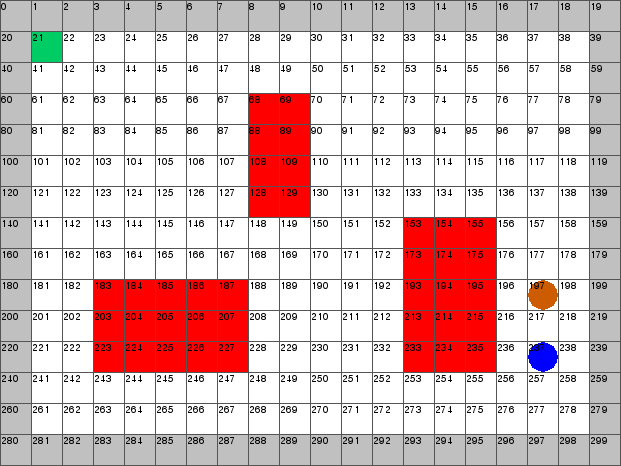
\includegraphics[scale=0.3]{case2.png}\caption{Gridworld representing an outdoor environment.}\label{fig:case2}
\vspace{-.5cm}
\end{figure}
Figure \ref{fig:case2} shows a gridworld of an 'outdoor' environment where the red blocks model buildings. The environment and resulting reactive controller was then simulated in ROS.
In this setting we enforce a belief safety specification $\square p_{30}$ in addition to infinitely often reaching the green cell. Formally, the specification we solve is $\square \lozenge p_{30} \wedge \square \lozenge goal$. 
A controller is synthesized with 6 abstract states. This demonstrates that even for larger grids, a coarse abstraction can be enough to obtain a controller.
 
 A video simulation can be found at \textbf{LINK}. Note the qualitative difference in behaviour. In the previous example, the agent had more leeway to completely lose the target in order to achieve the reachability specification even though the requirement of having to actually reduce the belief to 1 was stricter. However, in this example, due to the presence of the safety surveillance objective, the agent is forced to follow the target more closely in order to avoid having the belief grow too large. 
\Suda{Not sure if we should keep this next part}
\subsection{Discussion of behaviour}
The difference in the behaviour in the case studies highlights the different use cases of the surveillance objectives. In more indoor settings or structured environments, a liveness surveillance objective is feasible as the agent can more easily search and find the target even if the belief grows very large. However, in outdoor environments this is harder to accomplish as the target has more room to hide. 